\documentclass[11pt,a4 paper]{article}
\usepackage{amsmath, amsthm} 
\usepackage[english]{babel}
\usepackage[T1]{fontenc}
\usepackage[utf8]{inputenc}
\usepackage[margin=2cm]{geometry}
\usepackage{graphicx}
\usepackage{subfig}
\usepackage{caption}
\usepackage{siunitx}
\captionsetup{tableposition=top,font=small,width=0.8\textwidth}
\usepackage{booktabs}
\usepackage[table]{xcolor}
\usepackage[arrowdel]{physics}
\usepackage{mathtools}
\usepackage{tablefootnote}
\usepackage{amssymb}
\usepackage{enumitem}
\usepackage{multicol}
\setlist[description]{font={\scshape}} %style=unboxed,style=nextline
\usepackage{wrapfig}
\usepackage{float}
\usepackage{import}
\usepackage{floatflt}
\usepackage{url}
\usepackage{commath}
\usepackage{bm}
\usepackage[version=4]{mhchem}
\usepackage{nicefrac}
\usepackage{ifthen}
\usepackage{comment}
\usepackage[colorinlistoftodos,textsize=tiny]{todonotes}
\usepackage{hyperref}

\renewcommand*{\thefootnote}{\fnsymbol{footnote}}
\sisetup{exponent-product = \cdot}
\newcommand{\tc}{\,\mbox{tc}\,}
\newcommand{\Epsilon}{\mathcal{E}}
\newcommand{\half}{\frac{1}{2}}
\newcommand{\overbar}[1]{\mkern 1.5mu\overline{\mkern-1.5mu#1\mkern-1.5mu}\mkern 1.5mu}
\let\oldfrac\frac
\renewcommand{\frac}[3][d]{\ifthenelse{\equal{#1}{d}}{\oldfrac{#2}{#3}}{\nicefrac{#2}{#3}}}

\title{Positronium}
\author{Andrea Grossutti, mat. 1237344\\Alessandro Lovo, mat. 1236048\\Leonardo Zampieri, mat. 1237351}
\date{\today}

\begin{document}

\maketitle

\section{Aims}
\begin{itemize}
    \item Measure the ratio between the two and three photons decay of the Positronium;
    \item Measure the lifetime of the Positronium through the time distribution of the decays.
\end{itemize}

\section{Experimental setup}
The experimental setup consist in 4 inorganic scintillators; three coplanar (DET. 1,2,3) and a fourth (DET. 4) perpendicular to the plane.

The first three detector are placed on a circumference in the center of which lies a \ce{^22Na} source, with an activity of around $380\si{kBq}$. These detector are free movable around the circumference; in this session, two different configurations have been explored. To observe the two-photons decay, the detectors \#1 and \#2 have been aligned; instead, to observe the three-photons decay, the three coplanar detectors have been positioned to form an equilateral triangle.

Data are collected from the detectors through a electronic chain: a fan-in-fan-out quad module reply the signal of each detectors and produce four copies of it; then, through a CFD, a trigger signal is produced.  The CFD trigger threshold has been set so that the background noise is discarded, while the interesting signals produce an output. As can be seen from fig. \ref{fig:oscilloscope}, the signals corresponding to the detection of the $511\si{\kilo\electronvolt}$ and $1275\si{\kilo\electronvolt}$ photons are clearly visible.

\begin{figure}[H]
    \centering
    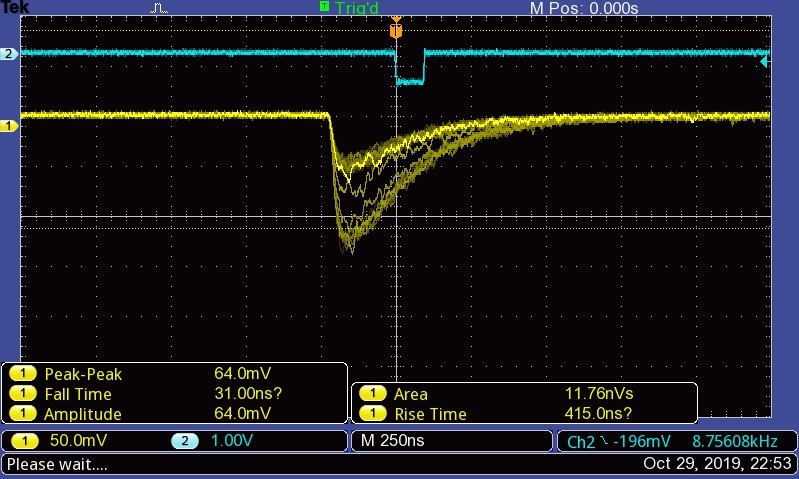
\includegraphics[width=0.7\textwidth]{img/TEK0001.JPG}
    \caption{Signal from the detector (yellow), triggering through the CFD (blu). The two different types of peaks, respectively for the $511\si{\kilo\electronvolt}$ and $1275\si{\kilo\electronvolt}$ photons, are clearly visible. Det. \#2.}
    \label{fig:oscilloscope}
\end{figure}

Between the second and the third day, a technical problem required the substitution of the high voltage power supply; due to this, thresholds have been re-set; moreover, in the middle of the day 3 the high voltage power supply burned; it has been replaced and the threshold re-set. While in the first two days all the detectors saw the two peaks around an amplitude of respectively $100$ and $250\si{\milli\volt}$ (and therefore the threshold has been set at about $75\si{\milli\volt}$), in the third day the detectors \#1 and \#3 saw the two peaks around an amplitude of respectively $50$ and $125\si{\milli\volt}$ (and therefore the threshold has been set at about $35\si{\milli\volt}$). For the detector \#4, finally, the threshold has been set to about $200\si{\milli\volt}$, such that only the higher energetic photons produce a trigger.

The CFD is provided of two sets of microswitches, to adjust delay and switch of the output signal. As has been verified thanks to the oscilloscope, the delay microswitches allow to adjust the time between the triggering of the system and the start of the logic signal, while the switch microswitches can be used to adjust the time length of the logic signal.

\section{Apparatus calibration}
Due to the various problem, the apparatus calibration has been done many times; only the first calibration is here reported, having for the other followed the same procedure.

The positions of the two peaks are know with very high precision:
\begin{table}[H]
    \centering
    \begin{tabular}{cccccccc}
        \toprule
        \ce{^22Na} Gamma radiations \\
        \midrule
        $511.0\si{\kilo\electronvolt}$ \\
        $1274.537\si{\kilo\electronvolt}$ \\
        \bottomrule
    \end{tabular}
    \caption{Gamma radiation for \ce{^22Na} from NuDat, \url{https://www.nndc.bnl.gov/nudat2/decaysearchdirect.jsp?nuc=22NA\&unc=nds}}
    \label{tab:gammavalue}
\end{table}

Acquiring the energy spectra with the digitizer, the two peaks are clearly visible; computing their centroids the horizontal axis can be linearly rescaled and be calibrated in energy. To fit the peaks, observing the variation of background before and after each peak, a gaussian plus a linear noise is:
\begin{equation*}
    f(x) = \underbrace{a + bx}_\text{noise} + \epsilon e^{-\frac[f]{(x-\mu)^2}{2\sigma^2}}
\end{equation*}

The following result are found:
\begin{table}[H]
    \centering
    \begin{tabular}{cccccccc}
        \toprule
        Det. & $\mu$ & $\sigma$ & $\chi^2/dof$ \\
        \midrule
        \#1 & $4345.0 \pm 0.1$ & $142.7 \pm 0.8$ & $107/80$ \\
        & $10589 \pm 2$ & $233 \pm 2$ & $137/149$ \\
        \#2 & $4679.4 \pm 0.6$ & $143 \pm 1$ & $150/80$ \\
        & $11362 \pm 2$ & $249 \pm 2$ & $140/159$ \\
        \#3 & $3304.3\pm0.5$ & $112.3\pm 0.7$ & $66/61$ \\
        & $8021\pm 1$ & $205\pm3$ & $118/108$ \\
        \#4 & $3303.0\pm0.4$ & $112.4\pm0.5$ & $102/67$ \\
        & $8021\pm1$ & $205\pm3$ & $118/108$\\
        \bottomrule
    \end{tabular}
    \caption{Interpolation results}
    \label{tab:calibr1}
\end{table}

The similarity between the chi-squared value and the number of degree of freedom for all the fits, combined with the observation of the fit plots, guarantee the reliability of the interpolations. For each detector the rescaling factor are computed and thus the resolution $r$.

\begin{gather*}
    E = a \cdot \text{channel} + b \\
    r = \frac{\text{FWHM}_E}{\mu_E} = 2\sqrt{2\ln2} \frac{\sigma_E}{\mu_E} = 2\sqrt{2\ln2} \frac{a \cdot \sigma_c}{a \cdot \mu_c + b} = 2\sqrt{2\ln2} \frac{\sigma_c}{\mu_c + \frac[f]{b}{a}}
\end{gather*}

\begin{table}[H]
    \centering
    \begin{tabular}{cccccccc}
        \toprule
        Det. & $a [\si{\kilo\electronvolt}]$ & $b [\si{\kilo\electronvolt}]$ & $r_1$ & $r_2$ \\
        \midrule
        \#1 & $0.12228\pm0.00004$ & $-20.3\pm0.2$ & $8.03\pm0.05$ & $5.25\pm0.05$ \\
        \#2 & $0.11426\pm0.00004$ & $-23.7\pm0.2$ & $7.54\pm0.05$ & $5.25\pm0.05$ \\
        \#3 & $0.16188\pm0.00004$ & $-23.9\pm0.2$ & $8.38\pm0.05$ & $6.12\pm0.09$ \\
        \#4 & $0.16183\pm0.00004$ & $-23.5\pm0.2$ & $8.38\pm0.05$ & $6.12\pm0.09$ \\
        \bottomrule
    \end{tabular}
    \caption{Calibration result}
    \label{tab:calib2}
\end{table}
The resolutions for the peaks are similar between the four detectors.

\begin{figure}[H]
    \centering
    \resizebox{0.8\textwidth}{!}{\import{img/}{det1_calibration.tex}}
    \caption{Calibration of detector 1: in blue the histogram of the detected signals, in red and green the peaks fits used for the calibration. Note the x axis properly calibrated in energy.}
    \label{fig:det1_calibr}
\end{figure}


Finally, even the TAC must be calibrated. This module return a voltage signal whose amplitude is proportional to the time difference between the triggering of the \emph{start} and the \emph{stop} channels. To calibrate it, the two channels are connected to the same signal; moreover, between the signal and the stop a delay module is inserted. Some measures are made with different delay, obtaining the following histograms (fig. \ref{fig:tachisto}).

\begin{figure}[H]
    \centering
    \resizebox{0.8\textwidth}{!}{\import{img/}{tac_calibr.tex}}
    \caption{Measure collected from the TAC, with different delay, in about $1\si{\minute}$ of acquisition in day \#2.}
    \label{fig:tachisto}
\end{figure}

Neglecting the zero-delay data (too close to the border of the histogram to efficiently find a centroid), centroids for the other peaks have been computed as the average of the registered values, with an associated error corresponding to the standard deviation of the data: a fit or a more precise statistic is meaningless due to the low number of channels in which data are spread on.  Having no a \emph{zero} point, i.e. even if the \emph{start} and the \emph{stop} signal are the same cables and other electronic device can introduce a delay between them, only difference can be meaningful defined. The calibration must be done separately for the $2\gamma$ and the $3\gamma$ detector: the range of the TAC used in the two detection has been chosen different, to optimize the data collecting. A linear fit on the centroids return the following results:

\begin{gather*}
    \Delta\text{channel}  = m \cdot \Delta t \\
    m_{2\gamma} = ( 117 \pm 1 )\si{\per\nano\second} \\
    m_{3\gamma} = ( 87.4 \pm 0.4 )\si{\per\nano\second}
\end{gather*}

\begin{figure}[H]
    \centering
    \resizebox{0.8\textwidth}{!}{\import{img/}{tac_calibr_fit.tex}}
    \caption{TAC calibration fit, for the $2\gamma$ setup.}
    \label{fig:tac_calibr_fit}
\end{figure}



\section{Digitizer dead time}
The digitizer has a dead time: when it is triggered, it takes some time to scan over all channel and register data. To estimate the dead time, during the three experimental days multiple test have been done, measuring the frequency of different signals with both the digitizer (counting the number of registered events over the acquisition time) and with a scaler module, which has a negligible dead time. The result founded are summarized in table \ref{tab:rate}.

\begin{table}[H]
    \centering
    \begin{tabular}{cccccccc}
        \toprule
        Event & Real rate [\si{Hz}] (scaler)& Measured rate [\si{Hz}] (digit.) \\
        \midrule
        Det. \#1 day 1& $9211 \pm 80$ & $6543 \pm 10$ \\
        Det. \#2 day 1& $12248 \pm 80$ & $5997 \pm 10$\\
        Det. \#1\&\#2 day 2& $3687 \pm 10$ & $3683 \pm 1$ \\
        Det. \#1\&\#2\&\#4 day 2& $44 \pm 1$ & $43.9 \pm 0.2$ \\
        Det. \#1 day 3& $12610 \pm 70$ & $7084 \pm 11$ \\
        Det. \#2 day 3& $12460 \pm 40$ & $6001 \pm 10$ \\
        %Coincidences det. \#1-\#2 & $4740 \pm 20$ & $$ \\
        Det. \#1\&\#2\&\#4 day 3& $60 \pm 3$ & $59.8 \pm 0.1$ \\
        \bottomrule
    \end{tabular}
    \caption{Event rate}
    \label{tab:rate}
\end{table}

\todo[inline]{Cercare se ci sono altri rate interessanti}

The PDF of the time between two consecutive decays follow an exponential distribution:
\begin{equation*}
    p(t) = \nu e^{-\nu t} \qquad \rightarrow \qquad <t> = \int_0^{\infty} tp(t) \dd{t} = \frac{1}{\nu}
\end{equation*}
where $\nu$ is the event frequency. If the system has a dead time, two event are discerned only if them differs of a time larger than the dead time $\tau$; the measured frequency is therefore:
\begin{equation*}
    \frac{1}{\nu^\star} = \frac{\int_{\tau}^{\infty} t p(t) \dd{t}}{\int_{\tau}^{\infty} p(t) \dd{t}} =\frac{\nu\tau + 1}{\nu}
\end{equation*}

\todo[inline]{Fit data and find $\tau$}

\section{Two photons events}

\begin{figure}[H]
    \centering
    \subfloat[][Placement of the detectors]
    {\def\svgwidth{0.4\textwidth}\import{img/}{rivel180.pdf_tex} \label{fig:rivel180:placement}} \quad
    \subfloat[][Electronic scheme]
    {\def\svgwidth{0.4\textwidth}\import{img/}{electro180.pdf_tex}}
    \caption{Two photons relevation.}
    \label{fig:rivel180}
\end{figure}

To detect the two-photons events, the detectors have been placed as in fig. \ref{fig:rivel180:placement}. The electronics have been set to be triggered with the coincidente between det. \#1, \#2 and \#4. However, we expect the detector \#4 to observe the photons shortly before the other two detectors, because of the lifetime of the positronium. To prevent \emph{false negative}, the width of the CFD of the detector \#4 has been set to an high value to produce a long logic signal.

Moreover, the system has been set to measure the time difference between the signal from det. \#1 and \#2 and from det. \#4. 

\todo[inline]{- Spettri energia calibrati (picchi 1 a 511, 2 a 511, 4 a 1275);}

Acquiring the time with TAC, what we obtain is the convolution of the decay law with the statistical error gaussian. At the end, what we see is a peaks centered in an arbitrary value (determined by the electronic configuration of the apparatus, the cable used and the delay introduced) which on the left shows a gaussian trend, while on the right the gaussian contribute is negligible and the exponential trend is visible. Fitting the right wing with an exponential is possible to find the parameters of the decay law, in particular the mean lifetime.

\todo[inline]{- Descrizione filtro - Spettro TAC filtrato e calibrato e fit expo}
\section{Three photons events}

\begin{figure}[H]
    \centering
    \subfloat[][Placement of the detectors]
    {\def\svgwidth{0.4\textwidth}\import{img/}{rivel120.pdf_tex} \label{fig:rivel120:placement}} \quad
    \subfloat[][Electronic scheme]
    {\def\svgwidth{0.4\textwidth}\import{img/}{electro120.pdf_tex}}
    \caption{Three photons relevation.}
    \label{fig:rivel120}
\end{figure}

To detect the three-photons events, the detectors have been placed as in fig. \ref{fig:rivel120:placement}. The optimal configurations would provide a triggering on the coincidences between all the four detectors. However, the three-photons events are very rare, and triggering on all the detectors would produce a too-low number of data to make a meaningful statistic, even with a full-night acquisition. Therefore the triggering has been set to the coincidences between the det. \#1, \#2 and \#3, making an a-posteriori coincidence with the detector 4 only for the timing studies.

\todo[inline]{- Spettro somma delle energie non filtrato - Spiegazione filtro + simulazioni - Spettri energie filtrati (somma + lowerbound + upperbound) (picchi 1,2 e 3 a 340); - Spettro TAC filtrato e discussione}

\section{Rate}

\todo[inline]{- Rate con le freq. di acquisizione opportunamente filtrate - simulazioni e conti spannomatrici per la rinormalizzazione dei rate e nuovi rate.}

\section{Conclusions}

\end{document}

